\documentclass[conference,compsoc]{IEEEtran}
\usepackage{paper-style}

\begin{document}

\title{Predicting Stock Prices \\ Using Machine Learning}

\author{\IEEEauthorblockN{Francesca Neri - 1018826}
\IEEEauthorblockN{francesca.neri26@studio.unibo.it}}

\maketitle

\begin{abstract}
The financial and banking sectors are incredibly data-rich, with millions of transactions and transfers occurring every day.
%
Machine learning models can be used to understand emerging and underlying trends in order to gain advantage in the financial sector. 

As any one of us could guess, the stock market is unstable and, more than often, unpredictable.
%
Of course, fundamental factors such as a company’s intrinsic value, assets, quarterly performance, recent investments, and strategies all affect the traders’ trust in the company and thus the price of its stock. 

Only a few of the latter can be incorporated effectively into a mathematical model, making stock price prediction challenging and unreliable to a certain extent.
\end{abstract}

\IEEEpeerreviewmaketitle

\section{Introduction}

Machine learning techniques can be used to make predictions about stock trends, but it is important to note that predicting stock prices is a challenging task, and no model or approach can guarantee accurate results.

It is also worth noting that the stock market is subject to a wide range of unpredictable factors, including changes in economic conditions, shifts in investor sentiment, and the impact of news events, which can all affect stock prices in ways that are difficult to predict. 
%
As a result, it is important to approach any predictions about stock trends with caution and to be prepared for the possibility that the actual results may differ from the predictions.

Most stock traders nowadays depend on Intelligent Trading Systems which use artificial intelligence and machine learning techniques to analyze financial data and make trading decisions.
%
There are a number of different approaches that can be used to build intelligent trading systems, including using historical data to train machine learning models, using technical analysis indicators to identify trends and patterns in the data, and using natural language processing techniques (NLP) to analyze news articles and other external data sources for insights into market movements.

When we talk about stock prediction, there are two approaches that can be used to analyze financial markets and make investment decisions, depending on the type of data we focus on and on the methods used to analyze those data.
%
One methodology - Fundamental analysis - involves analyzing a company's financial statements and other financial data, as well as its management, the company's competitive advantage and industry conditions, to try to determine the intrinsic value of its stock.
%
Technical analysis, on the other hand, involves analyzing historical price and volume data for a security or market to identify trends and patterns that may suggest buying or selling opportunities. 

When applying machine learning to stock data, we are more interested in doing a Technical Analysis as specific algorithms can be trained on historical price and volume data to identify patterns and trends that may not be immediately apparent to human analysts.

\section{Related Work}
There are a number of different approaches that have been used to try to predict stock trends using machine learning, including using historical stock price data, using news articles or other external data sources, and using technical analysis indicators as input features.

V. H. Shah in \textit{Machine Learning Techniques for Stock Prediction} highlighted the importance of relying on some key market theories and assumptions like the Efficient Market Hypothesis and the Random Walk Hypothesis \citep{shah2007machine}.

The Efficient Market Hypothesis states that financial markets are efficient and that prices reflect all available information about an asset.
%
According to the EMH, it is not possible for investors to consistently achieve returns above the average market return using the information that is publicly available, because prices already reflect all known information.

The Random Walk Hypothesis, on the other hand, states that stock price movements are independent of each other and are random.
%
According to this theory, stock price movements are the result of a large number of independent and unpredictable factors, such as changes in economic conditions, company performance, and investor sentiment.

Now a days, advanced intelligent techniques are used to deal with the huge size and variety of market data to identify hidden patterns and complex relations.
%
Most of the work in this area uses classical algorithms like linear regression, Moving Average Convergence / Divergence (MACD) \citep{linear}, linear models like Auto-regressive Moving Average (ARMA) and Auto-regressive Integrated Moving Average (ARIMA) \citep{arima} for predicting stock prices.

Recent work shows that stock market prediction can be enhanced using machine learning techniques such as Support Vector Machine, Random Forest, Artificial Neural Network, Convolutional Neural Network, Recurrent Neural Network and Deep Neural Networks \citep{neuron}.

Nabipour et al. conducted a research in which they focused on comparing the prediction performance of nine machine learning models (Decision Tree, Random Forest, Adaboost, XGBoost, SVC, Naïve Bayes, KNN, Logistic Regression and ANN) and two deep learning methods (RNN and LSTM) to predict stock market movements \citep{ieee}.
%
The study includes two different approaches for inputs, continuous data and binary data, to investigate the effects of pre-processing; the former uses stock trading data (open, close, high and low values) while the latter employs pre-processing steps to convert continuous data to binary ones.

Overall, the experimental works showed that there was a significant improvement in the performance of models when they use binary data instead of continuous ones. 
%
Indeed, deep learning algorithms (RNN and LSTM) were the superior models in both approaches.

\section{Data Understanding}
The purpose of this project is to predict the trend of the stock prices of NVIDIA corporation, an American multinational technology company which has been part of the S\&P 500 index since 2001 and its stocks are traded in the Nasdaq Stock Exchange as NVDA.
%
The data used in the project, imported from Yahoo Finance, are included in a single data frame indexed by date. 

\begin{figure}[h]
\centering
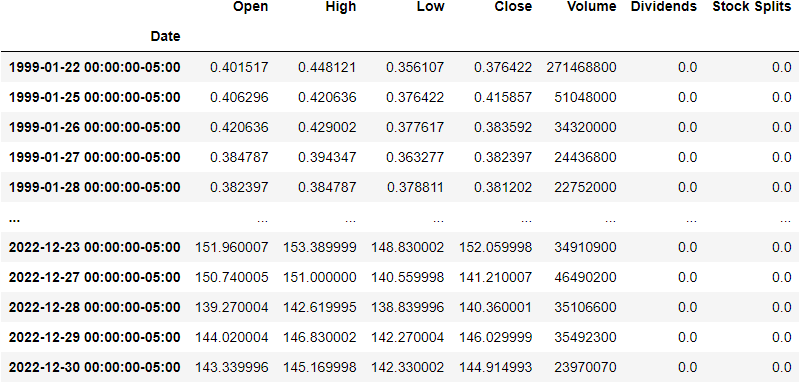
\includegraphics[width=3.3in]{images/dataframe.png}
\caption{Data frame with historical data}
\label{df}
\end{figure}

As we can see in figure \ref{df}, for each registered trading day, the data frame contains the details of the NVIDIA stock price movements.
%
In particular, the open value refers to the price at which the financial security opens in the market when trading begins, while the close value is the price at which the financial security closes in the market when trading ends.

The high value refers to the highest value at which the security was traded during a specific period while the low value is the lowest one.
%
The volume refers to the number of shares traded in a particular stock over a specific period of time, while stock splits refer to the corporate action that companies take to increase the number of outstanding shares and decrease the value of each share.

NVIDIA held its Initial Public Offering on January 22, 1999 so, by importing all the available historical data about the NVIDIA stock from the beginning until today, we will obtain a data frame with more than 6,000 instances (considering 252 trading days per year).

\begin{figure}[h]
\centering
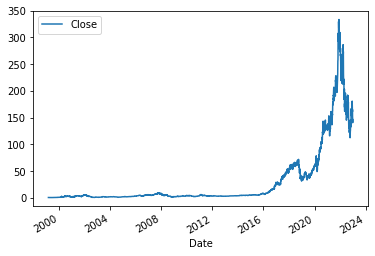
\includegraphics[width=3.3in]{images/trend.png}
\caption{Overall NVIDIA stock trend}
\label{trend}
\end{figure}

Figure \ref{trend} illustrates the stock price movements over 24 years, from 1999 until today.

Overall, the price remained stable until 2016 when it started increasing until it reached the highest price recorded of \$333.41 in November, 2021.
%
From that moment, it started decreasing and, in December 2022, the closing price oscillated from \$130 to \$170.

\section{Proposed Method}

In this section, we will see three different models that are all designed to predict the trend of the NVIDIA stock.
%
For each solution, we import the data about the stock from Yahoo Finance and, depending on the model, specific cleaning and transformation is applied to the data frame.

\subsection*{Bitcoin Model}

NVIDIA corporation gets the vast majority of its revenue from the sale of Graphic Processing Unit that can be used for gaming, cryptocurrency mining and professional applications.

It is worth noting that the demand for GPUs for cryptocurrency mining can sometimes lead to shortages and price increases for GPU producers, impacting the profitability of these latter.
%
NVIDIA GPUs are excellent for cryptocurrency mining and, according to Forbes, one of the most popular GPUs for mining is the NVIDIA GeForce GTX 1070 and 1080.

Following this idea, we designed a model aimed at predicting the NVIDIA stock trend by studying the trend of the stock of one of the most popular cryptocurrency: Bitcoin.

Bitcoin is a decentralized digital currency, created in 2009, that uses cryptography for security.
%
One of the main characteristics of Bitcoin is that it is decentralized, meaning that it is not controlled by any government, financial institution, or organization.
%
Instead, it relies on a network of computers that work together to verify transactions and add new ones to the block-chain.

\begin{figure}[ht]
\centering
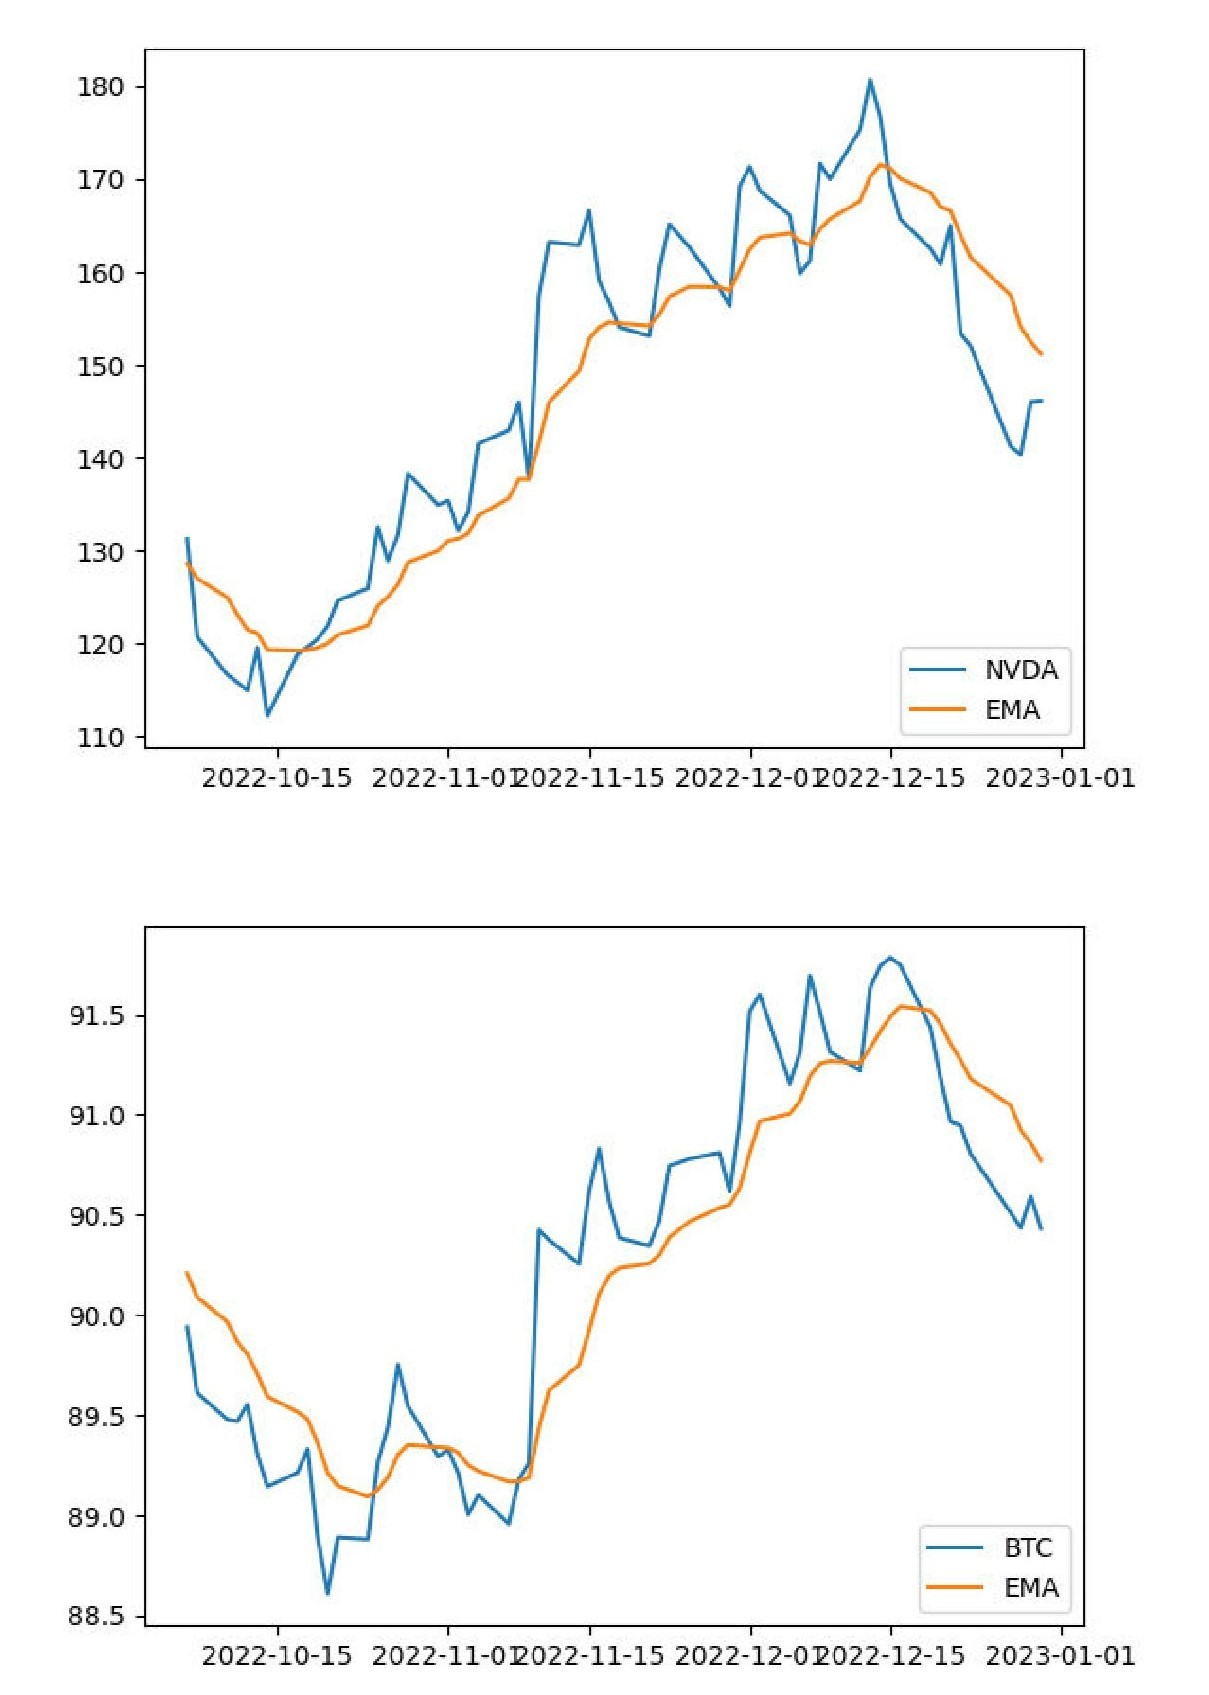
\includegraphics[width=3.3in]{images/nvidia-vs-bitcoin.jpg}
\caption{NVIDIA and Bitcoin stock trend using EMA}
\label{bitcoin}
\end{figure}

In figure \ref{bitcoin}, we compare the trend of both the NVIDIA and Bitcoin stock over the last 60 trading days.
%
To do so, we calculate the Exponential Moving Average (EMA) that is used in technical analysis to help smooth out price data and identify trends.

As it might be seen from the graph, we can spot some similarities in the EMA trend of NVIDIA and Bitcoin stocks.
%
Therefore, we can assume some degree of correlation between the two stocks and design a predictive model based on this aspect.

To design the model, we start by importing market data of both NVIDIA and Bitcoin from Yahoo Finance, which will be cleaned and transformed before analysis.
%
The data that we keep for the analysis include: open, high, low, close and volume.

Of course, the period for which historical data are available changes according to the stock selected.
%
Here, the available data for NVDA are significantly more compared to those for BTC.
% 
Therefore, we will keep only the most recent data about the NVIDIA stock so that the period analyzed is the same of Bitcoin.

Then, we create a new variable - \textbf{Target} - that is based on the following concept:

\begin{algorithmic}
    \State $t \gets today$
    \State $t1 \gets tomorrow$
    \If{$Close(t) \geq Close(t1)$}
        \State $Target \gets 0$ \Comment{Sell the stock}
    \Else
        \If{$Close(t) < Close(t1)$}
            \State $Target \gets 1$ \Comment{Buy the stock}
        \EndIf
    \EndIf
\end{algorithmic}

The target is calculated for both the stocks and the NVIDIA target is what we want our machine learning model to predict.
%
Since our target is binary (0 or 1), we will use a classification algorithm to try to predict the stock trend.

To reduce over-fitting, we shuffle data before splitting them into subsets.
%
To train the model, we will use 75\% of the whole data set, while model evaluation will be carried out with the remaining data (25\%).

\[ Model = Random Forest Classifier \]

Once the training and the test set have been defined, we initialize the Random Forest Classifiers with the following parameters:

\begin{itemize}
    \item n\_estimator = 100: number of individual decision trees that the algorithm should create
    \item min\_samples\_split = 100: minimum number of samples any decision tree should split on
    \item random\_state = 1: running the algorithm twice over the same data returns the same results
\end{itemize}

To check how accurate the model is, we will calculate its precision using the precision\_score function from scikit-learn.
%
Precision will tell us on what percentage of days that the algorithm said the price would go up, it actually went up. 
%
Because we want to minimize risk, we want to have a high precision so that when we buy stock, we have high confidence that we will make money.

For this model, the precision score ranges between 0.55 and 0.65.
%
Overall, accuracy is not great as, when the model predicted that prices would go up, they only went up 55\%-65\% of the time.

\subsection*{Technical Indicators}
Technical indicators are used by traders to gain insights into the supply and demand of securities and market psychology.
%
Together, these indicators form the basis of technical analysis. 

Metrics, such as trading volume, provide clues as to whether a price move will continue. 
%
In this way, indicators can be used to generate buy and sell signals.

For this model we will use all the available historical data about the stock, from 1999 until today.
%
Like in the previous model, we will keep only data about the open, close, high, low price and volume.

Also here, we calculate the target for each trading day (0 and 1) and the goal is to predict the target by studying some key technical indicators, which are respectively:

\begin{itemize}
    \item On Balance Volume (OBV)
    \item Accumulation Distribution Line (ADL)
    \item Average Directional Index (ADX)
    \item Relative Strength Index (RSI)
    \item Stochastic Oscillator (STOCH)
    \item Simple Moving Average (SMA)
\end{itemize}

\textbf{On-Balance Volume} (OBV) is a technical indicator that uses volume data to determine the buying and selling pressure of a security. 

As shown in the equation \ref{obv}, OBV is calculated by adding the volume of a security on up days (days when the price closes higher than the previous day) and subtracting the volume on down days (days when the price closes lower than the previous day).

\begin{equation} \label{obv}
    OBV = OBV_{prev} +
        \begin{cases}
            volume, & close > close_{prev}\\
            0, & close = close_{prev}\\
            -volume, & close < close_{prev}
        \end{cases}
\end{equation}

The idea behind OBV is that volume precedes price, so if the OBV is rising and the price of the security is flat or trending lower, it may be a sign of accumulation and a potential price increase in the future. 
%
Conversely, if the OBV is falling and the price of the security is flat or trending higher, it may be a sign of distribution and a potential price decrease in the future.

The \textbf{Accumulation Distribution Line} (ADL) is a volume-based indicator designed to measure the cumulative flow of money into and out of a security.
%
Like OBV, ADL is a cumulative volume-based indicator that seeks to identify divergences between the stock price and the volume flow. 

The \textbf{Average Directional Index} (ADX) can be used to identify the strength of a trend, as well as to identify potential trend reversals. 
%
A rising ADX may indicate that a trend is becoming stronger, while a falling ADX may indicate that a trend is losing strength. 
%
In addition, a sudden increase in the ADX may be a sign of a potential trend reversal.

\begin{equation} \label{rsi}
    RSI = 100 - \left [ \frac{100}{1 + \frac{avg.gain}{avg.loss}} \right ]    
\end{equation}

The \textbf{Relative Strength Index} (RSI) is a momentum indicator that is used to measure the strength of a security's price action. 
%
As shown in equation \ref{rsi}, RSI is calculated using the average of the security's gains and losses over a given period of time, and is plotted on a scale of 0 to 100.

The \textbf{Stochastic Oscillator} (STOCH) is a momentum indicator that compares the most recent closing price of a security to the highest and lowest prices during a specified period of time. 

The Stochastic Oscillator is often used to identify potential trend reversals and to confirm the strength of a trend. 
%
A rising Stochastic Oscillator may indicate that a security is gaining momentum and could potentially continue to trend higher, while a falling Stochastic Oscillator may indicate that a security is losing momentum and could potentially reverse its trend.

Finally, the \textbf{Simple Moving Average} (SMA) calculates the average of a selected range of prices, usually closing prices, by the number of periods in that range.

\begin{equation} \label{sma}
    SMA =   \frac{A_{1} +  A_{2} + ... +  A_{n}}{n}
\end{equation}

As we can see in the equation \ref{sma}, SMA is calculated by adding recent prices and then dividing that figure by the number of time periods in the calculation average.
%
SMA is widely used by traders as it smooths out volatility and makes it easier to view the price trend of a security.

Like in the previous model, we will use a classification algorithm to predict the stock trend.
%
In this case, the predictors of the model are all the technical indicators that we calculated together with the initial data (open, high, low, close, volume).

For this model, the data frame is particularly big as for each trading day, from 1999 until today, all the six technical indicators mentioned before are calculated.

We run the Random Forest Classifier with 100 estimator and 100 as the minimum number of splits.
%
Also here, we shuffle data and we train the model using 80\% of the data set and 20\% for the model evaluation.

The precision score ranges between 0.52 and 0.60, showing a lower accuracy compared to the first model.

\subsection*{Linear Regression}
Linear regression is a statistical method used to model the linear relationship between a dependent variable and one or more independent variables.
%
The goal of linear regression is to find the values of the coefficients that best fit the data, which is done by minimizing the sum of the squared differences between the observed values of the dependent variable and the values predicted by the equation.

Stock market forecasting is an attractive application of linear regression but the challenging aspect regards finding the right combination of features to make those predictions profitable.

In this model, we import all the available historical data about the NVIDIA stock but we keep only the closing price (indexed by date).
%
The goal is to predict the closing price using the Exponential Moving Average (EMA).

This type of moving average gives more weight to recent prices and less weight to older prices.
%
It is calculated using a specific formula that involves a smoothing constant, which determines the weight given to the most recent price.
%
The smoothing constant is usually set to a value between 0 and 1, with higher values giving more weight to the most recent price.

As we can see in figure \ref{ema}, the EMA smooths out short-term fluctuations in data and highlight long-term trends.
%
In this model, the data set that we will use for the analysis is composed by the closing price of the NVIDIA stock, from the oldest to the latest value available, and, for each trading day, the Exponential Moving Average.

\begin{figure}[ht]
\centering
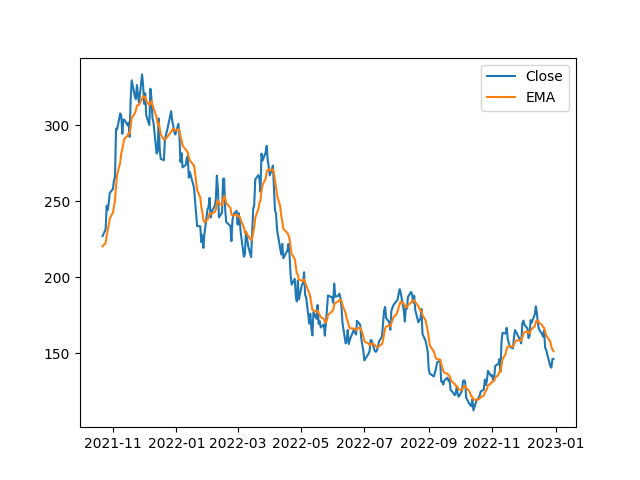
\includegraphics[width=3.3in]{images/ema.png}
\caption{NVIDIA stock EMA and closing price}
\label{ema}
\end{figure}

Before initializing the model, we split the data set in train set (80\%) and test set (20\%) that will be fit to the linear model.

\[ Model = Linear Regression \]

Once the train set and the test set have been defined, we run the linear regression model which will generate coefficients for each feature during training and returns these values as an array.
%
To assess how well the model fits the data, we can examine the model coefficients and some statistics like standard deviation (SD), the Mean Absolute Error (MAE) and the coefficient of determination (r2).

The \textbf{standard deviation} (SD) is a measure of the amount of variation or dispersion of a set of values.
%
A low standard deviation indicates that the values tend to be close to the mean, while a high standard deviation indicates that the values are spread out over a broader range.

\begin{equation} \label{sd}
    \sigma = \sqrt{\frac{\sum_{{i = 1}}^{N}(x_{i} - \mu)^2}{N - 1}}
\end{equation}

As shown in equation \ref{sd}, standard deviation is calculated as the square root of the variance, which is the average of the squared differences between the values and the mean of the values.

The \textbf{Mean Absolute Error} is calculated as the average of the absolute differences between the predicted values and the actual values, over all the data points in the data set. 
%
Mathematically, it is represented as:

\begin{equation} \label{mae}
    MAE = \frac{\sum_{i = 1}^{N}\left| y_{i} - x_{i} \right|}{N}
\end{equation}

MAE is a measure of errors between paired observations expressing the same phenomenon which, in our model, compares predicted values and observed values.

The \textbf{Coefficient of Determination} (r2) is a statistical measure that represents the proportion of the variance for a dependent variable that is explained by an independent variable in a regression model. 

\begin{equation} \label{r2}
    R^2 = 1 - \frac{\sum_{i = 1}^{N}(\widehat{y_{i}} - y_{i})^2}{\sum_{i = 1}^{N}(y_{i} - \overline{y_{i}})^2}
\end{equation}

R-squared explains to what extent the variance of one variable explains the variance of the second variable. 
%
As shown in equation \ref{r2}, the coefficient of determination is calculated by dividing the sum of squares of residual by the total sum of squares.

For this model, standard deviation amounts to 59, meaning that data are rather spread out, while the Mean Absolute Error amounts to 1, so the average distance from the predicted value and the true value is 1. 
%
The coefficient of determination of the model amounts to 0.99 which indicates that the the regression model fits well the observations. 

\section{Conclusions}
The results of the analysis are summarized in table \ref{results} which, for each model, specifies the level of accuracy and the evaluation metrics.

\begin{table}[ht]
\renewcommand{\arraystretch}{1.3}
\caption{Results of the Analysis}
\label{results}
\centering
\begin{tabular}{|m{8em}|m{8em}|m{8em}|}
    \hline
    \textbf{Name} & \textbf{Model} & \textbf{Accuracy}\\
    \hline
    Bitcoin & Random Forest & 55\%-65\% \\
    \hline
    Tech. Indicators & Random Forest & 52\%-60\% \\
    \hline
    Linear Regression & Linear Regression & std = 59, MAE = 1, r2 = 0.99 \\
    \hline
\end{tabular}
\end{table}

As we can see from the table, the overall accuracy for the first two models is not remarkably high.
%
In particular, if we consider that the target to be predicted is binary (0 or 1), an accuracy level of 60\%-65\% over a natural probability of 50\% is not that great.

Possible reasons for this low accuracy may be the lack of data and, of course, using a very simple model to perform such a complex task as stock market prediction.
%
To improve the algorithm, some of the steps that can be pursued, include:

\begin{itemize}
    \item Discard old data and focus only on a certain time window
    \item Try different machine learning algorithm like artificial neural networks
    \item Add more predictors 
\end{itemize}

While for what concerns the linear regression model, we need to discuss a technical limitation of this statistical model.
%
Linear regression requires a series of assumptions to be validated in order to be effective:

\begin{itemize}
    \item Linearity: the relationship between the predictor variables and the response variable is linear.
    \item Independence: the errors (residuals) are independent of each other.
    \item Homoskedasticity: the errors (residuals) have constant variance.
    \item Normality: the errors (residuals) are normally distributed.
    \item Absence of multicollinearity: the predictor variables are not highly correlated with each other.
\end{itemize}

The assumption of independence among residuals can be problematic in our model as we are dealing with time-series data which may show a seasonality trend.

The metrics here suggests that the model fits well the data but we need to keep in mind that the R-squared may be a biased estimate and the model may be over-fitting. \\

In conclusion, machine learning is an incredibly powerful technique to create predictions using historical data, and the stock market is a great application of that. 

However, it is important to note that the stock market is often very unpredictable and technical analysis should always be followed by fundamental analysis.
%
Moreover, it is nearly impossible to anticipate a piece of news that will shatter or boost the stock market in the coming weeks, like a global pandemic or a war.

Even if hundreds of variables and real-world market drivers are quantified, incorporated in the data and optimized using the best machine learning methods available, the model would still fall short of making valuable predictions when they matter.

Experts note that AI models could not follow the trends disrupted by the COVID-19 pandemic – not during or even towards the end of it \citep{forbes}.

In predictive models, most of the value comes from the input variables or underlying drivers that have information to predict output variables instead of the chosen model. 
%
Therefore, it becomes extremely important to choose input variables based on human intelligence or economic intuition and not just rely on data.

\bibliographystyle{plainnat}
\bibliography{bibliography}

\end{document}


